\documentclass[twocolumn]{article}
\usepackage{longtable}
\usepackage{graphicx}
\usepackage{lipsum}
\usepackage{hyperref}
\usepackage{amsmath, amssymb}
\usepackage[style=numeric-comp,useprefix,hyperref,backend=bibtex]{biblatex}
\graphicspath{{../img/}}
\usepackage{endnotes}
\usepackage{float}
\title{Wine Project Report}
\author{Ruggero Nocera (SXXXXX1) \\ Quarta Matteo (SXXXXXX)}
\date{}


\begin{document}

\maketitle
\tableofcontents


\section{Preliminary Data Analysis}
\subsection{Feature Distribution}

Before discussing the varius models and techniques that can give us robust result, we shortly discuss how the feature of our dataset are distributed.

\begin{figure}[H]
    \caption{Histogram of Class' Features}
    {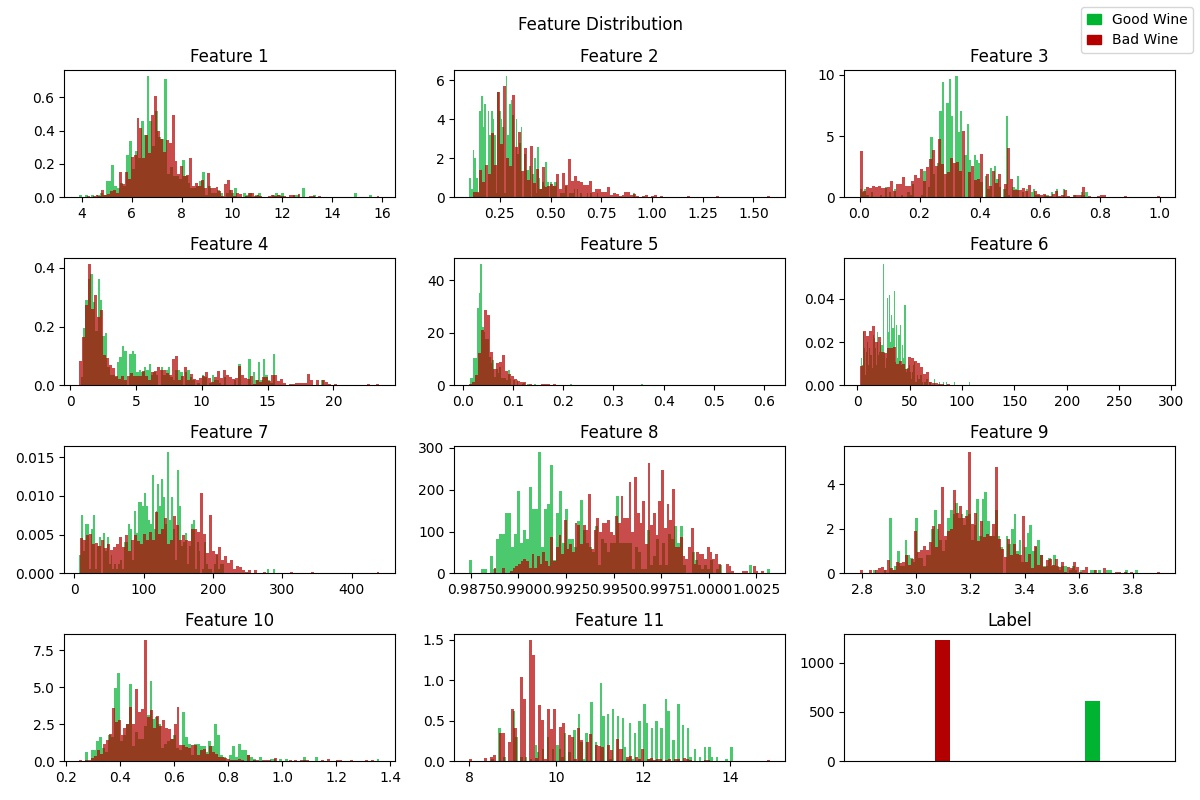
\includegraphics[width=\linewidth]{dist.jpg}}
    \label{featureshist}
\end{figure}

We start by noticing that the order of magnitude of some features can differ much from one another: for example, if we look at feature 5, it seems to span from 0.0 to as much as 0.6, but feature 7 instead spans two whole orders, occasionally being over 200, and with some outliers even double as much. An interesting observation is that some features do look gaussian distributed or regular enough to be described by a combination of gaussian distributions.

This may hint that some dimensionality reduction will be strongly biased towards features like 7, and that normalization can be taken as a valid pre-processing technique.

We also notice that our dataset is unbalanced: the quantity of bad wine is roughly twice the quantity of good one. This has to be taken into account when developing models, but we will be trating them as if the dataset is balanced, that is considering and equal probability of good wine and bad wine, occasionally rebalancing scores.

Let's apply a 2D projection of our data to further discuss it.

\begin{figure}[H]
    \caption{2D-PCA Projection}
    {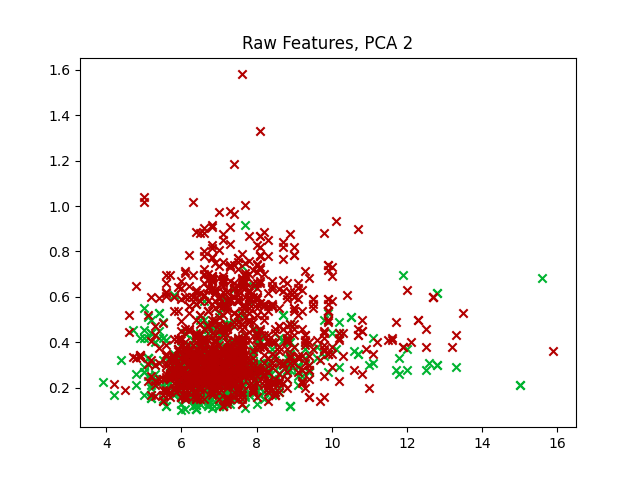
\includegraphics[width=\linewidth]{2DRAW.png}}
    \label{2DRAW}
\end{figure}

The features look highly correlated and fairly regularly distributed: this may be a hint that some gassuain models may perform well enough, like Full-Covariang MVG Classifiers or Tied-Covariance ones, but some other with linear decision boundaries, like linear SVMs, may perform poorly.

\begin{figure}[H]
    \caption{2D-PCA Projection, Normalized Data}
    {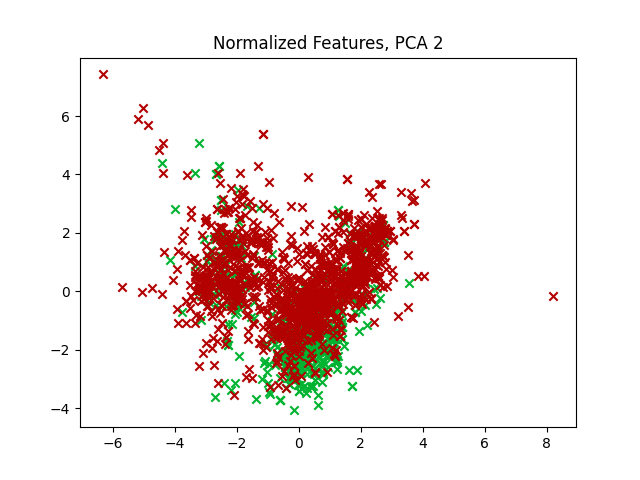
\includegraphics[width=\linewidth]{2DNorm.png}}
    \label{2DNORM}
\end{figure}

After normalization (Z-Normalization, mean $\mu = 0$ and St.D. $\sigma = 1$ ) our points do get apart but not significantly: we could expect linear models to still perform poorly and gaussian classifiers to get slightly worse. On the other hand, Gaussian Mixture Models look like a more interesting choice.

Lastly we take a look at normalized and whitened data.

\begin{figure}[H]
    \caption{2D-PCA Projection, Whitened Data}
    {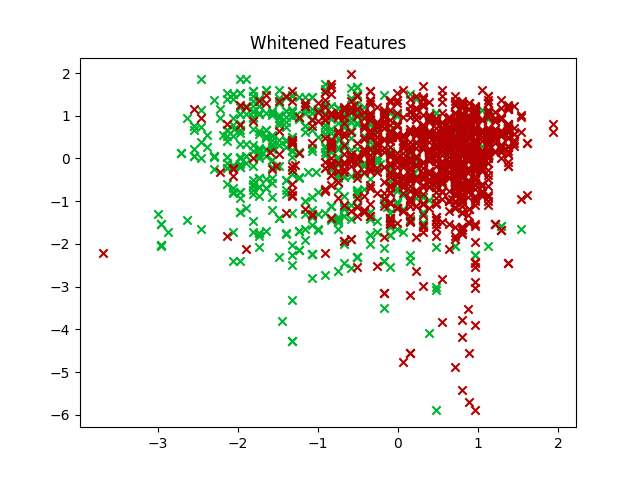
\includegraphics[width=\linewidth]{2DWhitened.png}}
    \label{2DWHI}
\end{figure}

Here the results are a bit more interesting: points do get separeted just like after normalization, but same class points stay close to each other while different class get more apart. In this scenario, it looks like even linear model might have a chance to achieve a decent performance.

\subsection{Dimensionality Reduction}

We will shortly decide, by running some non-optimized models, which pre-processing techniques are useful and which are not. 

We will be reporting the best results for each classifiers, extracted from a 3 or 5 Fold Validation approach. The decision rule, since this is a binary problem, will be set to $\displaystyle t = \log(\frac{\pi_T}{1-\pi_T}) \lessgtr 0 $, where $\pi_T$ is assumed $ = 0.5$ and it is the prior probability of class Good.

Let's start with Gaussian Classifiers: Full-Covariance, Tied-Covariance, and Naive-Bayes.


    \begin{table}
    \begin{tabular}{||c|c|c||}
        \hline
        PCA & DCF & minDCF \\
        \hline
        \hline
        A & B & C \\
        A & B & C \\
    \end{tabular}
\end{table}
\caption{My Table}



% Logistic Regression results
\newpage
\begin{table}
\begin{center}
\begin{tabular}{|c|c|}
\hline
$\lambda$ & Error Rate \\
\hline
0 & 16.026\% \\
\hline
1e-09 & 16.081\% \\
\hline
1e-06 & 16.081\% \\
\hline
0.001 & 15.587\% \\
\hline
0.1 & 18.057\% \\
\hline
\hline
\end{tabular}
\end{center}
\caption{Logistic Regression}\label{tab:logreg}

\begin{center}
\begin{tabular}{|c|c|c|}
\hline
$\lambda$ & PCA & Error Rate \\
\hline
0.001 & 10 & 15.587\% \\
\hline
0 & 8 & 15.862\% \\
\hline
1e-09 & 8 & 15.862\% \\
\hline
1e-06 & 8 & 15.862\% \\
\hline
0.001 & 8 & 15.917\% \\
\hline
0 & 10 & 16.081\% \\
\hline
1e-09 & 10 & 16.081\% \\
\hline
1e-06 & 10 & 16.136\% \\
\hline
0 & 6 & 16.630\% \\
\hline
1e-09 & 6 & 16.630\% \\
\hline
\end{tabular}
\end{center}
\caption{Logistic Regression With PCA}\label{tab:logreg_pca_acctable}

\begin{center}
\begin{tabular}{|c|c|c|}
\hline
$\lambda$ & PCA & Error Rate \\
\hline
0.001 & 10 & 15.038\% \\
\hline
0 & 10 & 15.258\% \\
\hline
1e-09 & 10 & 15.258\% \\
\hline
1e-06 & 10 & 15.258\% \\
\hline
0 & 8 & 15.532\% \\
\hline
1e-09 & 8 & 15.532\% \\
\hline
1e-06 & 8 & 15.532\% \\
\hline
0.001 & 8 & 15.532\% \\
\hline
0.001 & 6 & 16.246\% \\
\hline
0 & 6 & 16.301\% \\
\hline
\end{tabular}
\end{center}
\caption{Logistic Regression With PCA and Z-Normalization}\label{tab:logreg_pcan_acctable}

\end{table}

% Linear SVM results
\newpage
\begin{table}
\begin{center}
\begin{tabular}{|c|c|c|}
\hline
Bias & $C$ & Error Rate \\
\hline
0 & 0.1 & 17.728\% \\
\hline
0 & 1 & 16.520\% \\
\hline
1 & 0.1 & 35.565\% \\
\hline
1 & 1 & 38.090\% \\
\hline
5.0 & 0.1 & 15.862\% \\
\hline
5.0 & 1 & 47.805\% \\
\hline
10.0 & 0.1 & 15.642\% \\
\hline
10.0 & 1 & 16.081\% \\
\hline
\hline
\end{tabular}
\end{center}
\caption{Linear SVM}\label{tab:svm_linear_acctable}

\begin{center}
\begin{tabular}{|c|c|c|c|}
\hline
Bias & $C$ & PCA & Error Rate \\
\hline
10 & 0.1 & 10 & 15.313\% \\
\hline
5 & 0.1 & 10 & 15.642\% \\
\hline
5 & 0.1 & 6 & 15.971\% \\
\hline
10 & 0.1 & 8 & 16.301\% \\
\hline
5 & 0.1 & 8 & 16.356\% \\
\hline
10 & 0.1 & 6 & 16.575\% \\
\hline
0.1 & 0.1 & 8 & 18.057\% \\
\hline
0.1 & 0.1 & 6 & 18.222\% \\
\hline
0.1 & 0.1 & 10 & 18.551\% \\
\hline
0 & 0.1 & 8 & 18.716\% \\
\hline
\end{tabular}
\end{center}
\caption{Linear SVM With PCA}\label{tab:svm_linpca_acctable}

\begin{center}
\begin{tabular}{|c|c|c|c|}
\hline
Bias & $C$ & PCA & Error Rate \\
\hline
1 & 0.1 & 10 & 14.709\% \\
\hline
5.0 & 0.1 & 10 & 14.929\% \\
\hline
10.0 & 0.1 & 10 & 14.929\% \\
\hline
1 & 1 & 10 & 15.038\% \\
\hline
5.0 & 1 & 10 & 15.038\% \\
\hline
10.0 & 1 & 10 & 15.038\% \\
\hline
1 & 1 & 8 & 15.258\% \\
\hline
5.0 & 0.1 & 8 & 15.258\% \\
\hline
5.0 & 1 & 8 & 15.258\% \\
\hline
10.0 & 0.1 & 8 & 15.258\% \\
\hline
\end{tabular}
\end{center}
\caption{Linear SVM With PCA and Z-Normalization}\label{tab:svm_linpcan_acctable}

\end{table}
\end{document}